\documentclass{article}
\usepackage{graphicx}
\usepackage{hyperref}
\usepackage{listings}
\usepackage{xcolor}
\usepackage{tikzsymbols}
\usepackage{float}

\lstset{
    basicstyle=\ttfamily,
    backgroundcolor=\color{gray!30},
}

\begin{document}

\graphicspath{ {./Images/} }
\tableofcontents

\section{Introduction}
Hello and welcome to Windows. This document describes the process of configuring windows machines to run on Proxmox. If you would like to add something, please contribute in the github.

\section{Getting the correct ISOs to Proxmox}
The goal is to get both the Windows Server and the VirtIO driver iso files onto proxmox.

You should can either download the files to your computer and then to proxmox, or you can have proxmox download them from "download from url."

In either case, the Windows Server 2019 iso is \href{http://www.microsoft.com/en-us/evalcenter/download-windows-server-2019
}{here} and the VirtIO iso is \href{https://fedorapeople.org/groups/virt/virtio-win/direct-downloads/stable-virtio/}{here}.

The VirtIO is necessary because proxmox says so (update with better reasoning). \href{https://pve.proxmox.com/wiki/Windows_VirtIO_Drivers#Windows_OS_Support}{Proxmox Wiki: Windows VirtIO Drivers}

VirtIO also enables the QEMU Guest Agent, which allows for many convenient things in proxmox.

\begin{figure}[h]
    \centering
    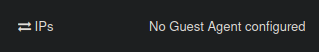
\includegraphics[width=0.5\textwidth]{noGuestAgent.png}
    \caption{The IP Address is not displayed if there is no guest agent}
    \label{fig:noGuestAgent}
\end{figure}

\section{Getting the VM from the ISO}
The goal is to take your .iso file and turn it into a VM. If it is helpful, here is some guy doing it with no words: \href{https://www.youtube.com/watch?v=lwORpWEHiDE&t=5m}{video} 

\noindent If you don't want to watch that, click "create VM" and select the iso file you uploaded.
\noindent The important settings to change are:
\vspace{1cm}

\begin{tabular}{l l}
    Category & Setting to Change\\
    \hline
    OS Type & Microsoft Windows, Version: 10/2016/2019 \\
    System & SCSI Controller: VirtIO SCSI Single \\
    System & QEMU Agent checked \\
    Disks & Bus/Device: SCSI \\
    Network & Bridge: (the Cyber Range Bridge, for me it is vmbr0)
  \end{tabular}

IMPORTANT: After creating this VM, click it and go to the “Hardware” menu in Proxmox. Click “add CD/DVD” and click the virtIO.iso file you uploaded. This will enable the QEMU Agent.

\section{Installing / Logging Into the VM}
Note: You can not use many of proxmox's features (i.e. shut it down without going through the console) without the guest agent installed. Just to save you from mashing the "shutdown" button and wondering why it doesn't work. 

\noindent How to get into the VM:

\begin{enumerate}
    \item Power on the VM
    \item Log onto the VM via the Proxmox console
\end{enumerate}

\noindent How to install Windows on the VM:

\begin{enumerate}
    \item Select "next"
    \item Select "2019 Standard Evaluation (Desktop Experience)"
    \item Select "Advanced Installation"
    \item Add the VirtIO driver you installed previously
\end{enumerate}

Now you wait for it to install. Don't worry, you'll get used to waiting for windows!

\section{Basic Configurations to Prepare for a Template}
The goal is to never do that time consuming process again. We would like to create a template so we can clone it. Before you make a template you can add useful things like RDP, Firefox, setting DNS, etc. The world is your oyster.

\subsection{Enabling RDP}

Bing can handle this one.

\begin{figure}[H]
    \centering
    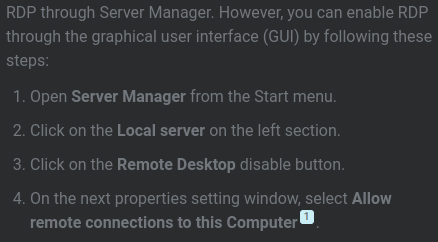
\includegraphics[width=1\textwidth]{bingDirectionsForEnableRDP.png}
    \caption{Bing explaining how to enable RDP}
    \label{fig:bingDirectionsForEnableRDP}
\end{figure}

\begin{figure}[H]
    \centering
    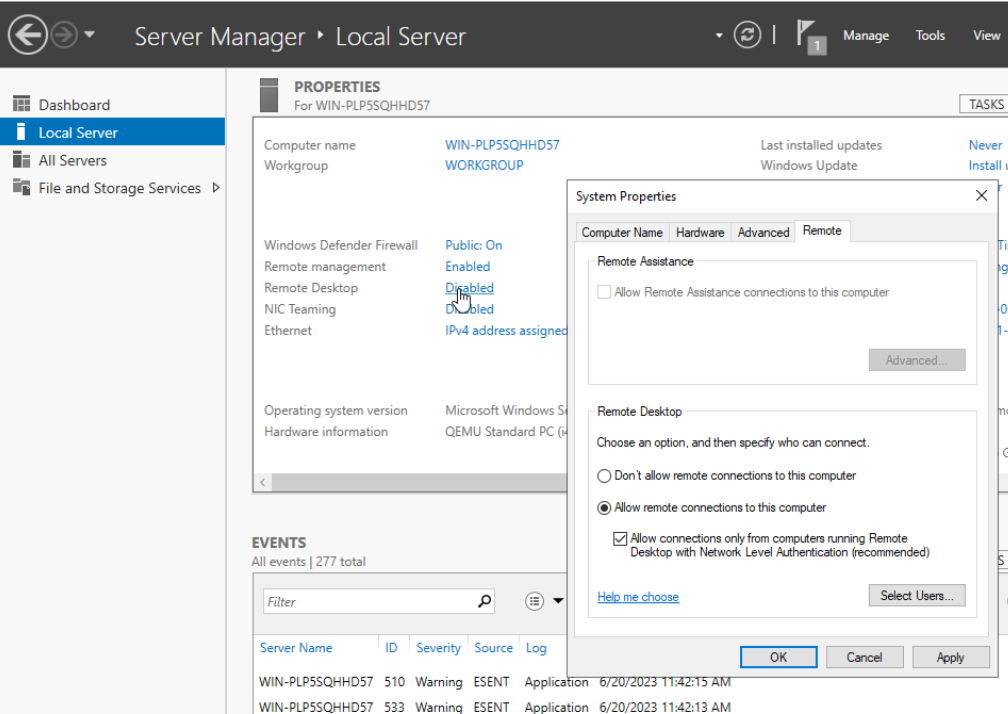
\includegraphics[width=1\textwidth]{enableRDP.png}
    \caption{Enabling RDP}
    \label{fig:enableRDP}
\end{figure}

\subsection{Installing Firefox}
By default, Internet Explorer is the only browser installed on the computer. What a terrible browser! You can avoid ever opening IE by installing Firefox from powershell. 
\begin{lstlisting}[breaklines=true, columns=fullflexible]
Invoke-WebRequest -Uri `
"https://download.mozilla.org/?product=firefox-msi-latest-ssl&os=win64&lang=en-US" `
-OutFile "$HOME\Desktop\firefox.msi"
    
\end{lstlisting}
        

\noindent This command saves firefox.msi to your desktop. Remember that you can download stuff from powershell. (But pls no proprietary browsers \Vomey{})

\noindent If the pdf messes up some part of the command, you can copy it from the latex file

\subsection{Setting up the QEMU Agent}
There are two steps. First, run the QEMU Agent installer. Second, add the VirtIO driver in the Device Manager.

Once you finish, the IP Address is visible from the “Summary” tab in proxmox. Very nice.

\begin{figure}[H]
    \centering
    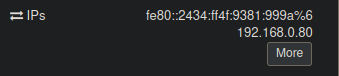
\includegraphics[width=1\textwidth]{successfulAgentIPThingie.png}
    \caption{IP Address in Proxmox}
    \label{fig:successfulAgentIPThingie}
\end{figure}

\subsubsection{Running the QEMU Agent Installer}
“In the Windows VM, open the File Explorer and navigate to the VirtIO driver ISO. Open the “guest-agent” folder and double-click on the “qemu-ga-x86\_64.msi” file to run the installer” -Bing

\begin{figure}[H]
    \centering
    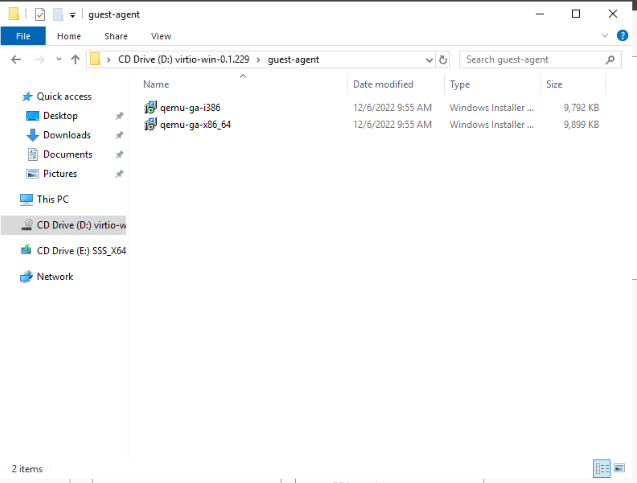
\includegraphics[width=1\textwidth]{runningGuestAgent.png}
    \caption{The MSI file to run}
    \label{fig:runningGuestAgent}
\end{figure}

\subsubsection{Adding VirtIO in Device Manager}

\begin{figure}[H]
    \centering
    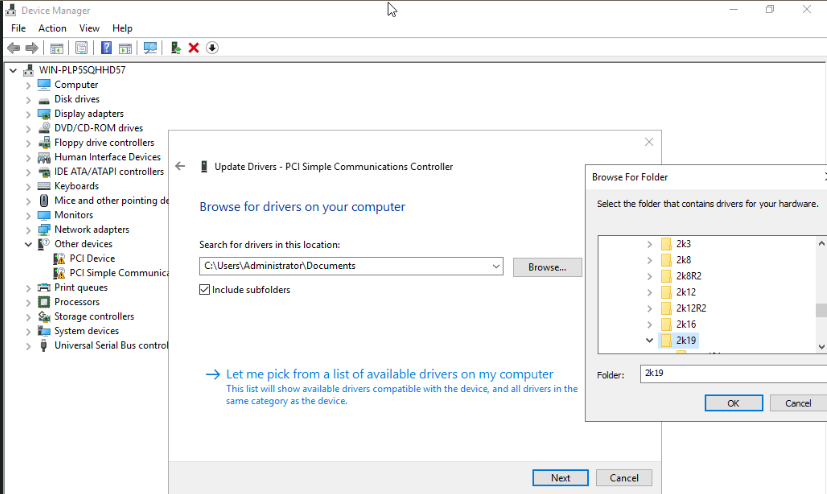
\includegraphics[width=1\textwidth]{Adding-VIRTIO-Driver.png}
    \caption{Selecting the 2k19 driver in the vioserial folder in the virtio CD drive.}
    \label{fig:Adding-VIRTIO-Driver}
\end{figure}

\subsection{Adding DNS Servers}

\subsection{Sysinternals}

\subsection{SIDCHG}

\begin{figure}[H]
        \centering
        \includegraphics[width=1\textwidth]{SIDError.png}
        \caption{Two machines have the same SID}
        \label{fig:SIDError}
\end{figure}

Cloning a template has issues because the SID (Security Identifier) of the cloned and original machines are the same.
There are probably smarter ways to get around a non-unique SID (e.g. using )

\begin{figure}[H]
        \centering
        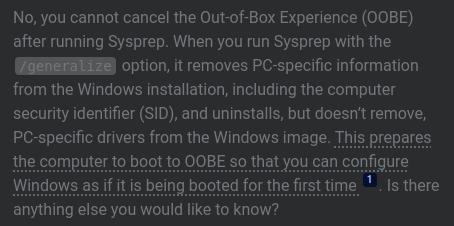
\includegraphics[width=1\textwidth]{dangersOfSysprep.png}
        \caption{You cannot cancel Sysprep once you start it}
        \label{fig:dangersOfSysprep}
    \end{figure}

Don’t be like me. Don’t run utilities you don’t understand because bing told you to!
If you run Sysprep, it will wipe your computer and you cannot get back into it. (or I probably just did it wrong...)

\noindent The program "SIDCHG" has worked for me. (SIDCHGL is easier as you don't have to disable your antivirus)
It should be installed on the template machine as all of the cloned machines will need to change their SID.

Go to: \href{https://www.stratesave.com/html/downloads.html}{stratesave.com/downloads}
and download the latest version of SIDCHG
In addition, you will also need the guy's free trial key, found at \href{https://www.stratesave.com/html/downloads.html}{stratesave.com/stupid\_key}

For more information, watch this \href{https://www.youtube.com/watch?v=4fImvgWayI0}{tutorial}

\subsection{An Anti-Virus}

I think the rules say to use only free/publicly available programs.
Windows Defender is good, but we can probably use a better antivirus.
I have heard good things about Kaspersky Free (even though the feds say otherwise)

I think I will use either BitDefender or Kaspersky. BitDefender seems much faster.
Can also give Kaspersky a password? Seems useful "you can set up a password to access kaspersky application settings making it harder someone else to change settings or disable the protection. I like its' customizable options,also like its password manager."
- youtube comment

\end{document}
